\documentclass{article}
\usepackage[utf8]{inputenc}
\usepackage[greek,english]{babel}
\usepackage{alphabeta}
\usepackage{graphicx}
\usepackage{hyperref} 
\usepackage{listings}
\usepackage{subcaption}
\usepackage{mathtools}
\usepackage{tikz}
\usepackage{multirow}
\date{}

















\begin{document}

\begin{titlepage} % Suppresses displaying the page number on the title page and the subsequent page counts as page 1
	
	\raggedleft % Right align the title page
	
	\rule{1pt}{\textheight} % Vertical line
	\hspace{0.05\textwidth} % Whitespace between the vertical line and title page text
	\parbox[b]{0.75\textwidth}{ % Paragraph box for holding the title page text, adjust the width to move the title page left or right on the page
		
		{\Huge\bfseries Τεχνικές \\ \\
		Βελτιστοποίησης\\ \\ }\\[2\baselineskip] % Title
		{\large\textit{ }}\\[4\baselineskip] % Subtitle or further description
		{\Large\textsc{Ιωάννης-Παναγιώτης \\Μπουντουρίδης}} %
	\\	\\{\large\textsc{ΑΕΜ: 8872}} % Author name, lower case for consistent small caps
		
		\vspace{0.5\textheight} % Whitespace between the title block and the publisher
		
		{\noindent \textit{work 2}}\\[\baselineskip] % Publisher and logo
	}

\end{titlepage}
\newpage
   
\section*{Θέμα 1 }

Γραφική παράσταση της συνάρτησης 
\begin{equation*}
f(x,y) = x^3 \cdot e^{-x^2-y^4}
\end{equation*}
\begin{figure*}[h!]	
     \centering  
     \advance\leftskip-0.2cm  
  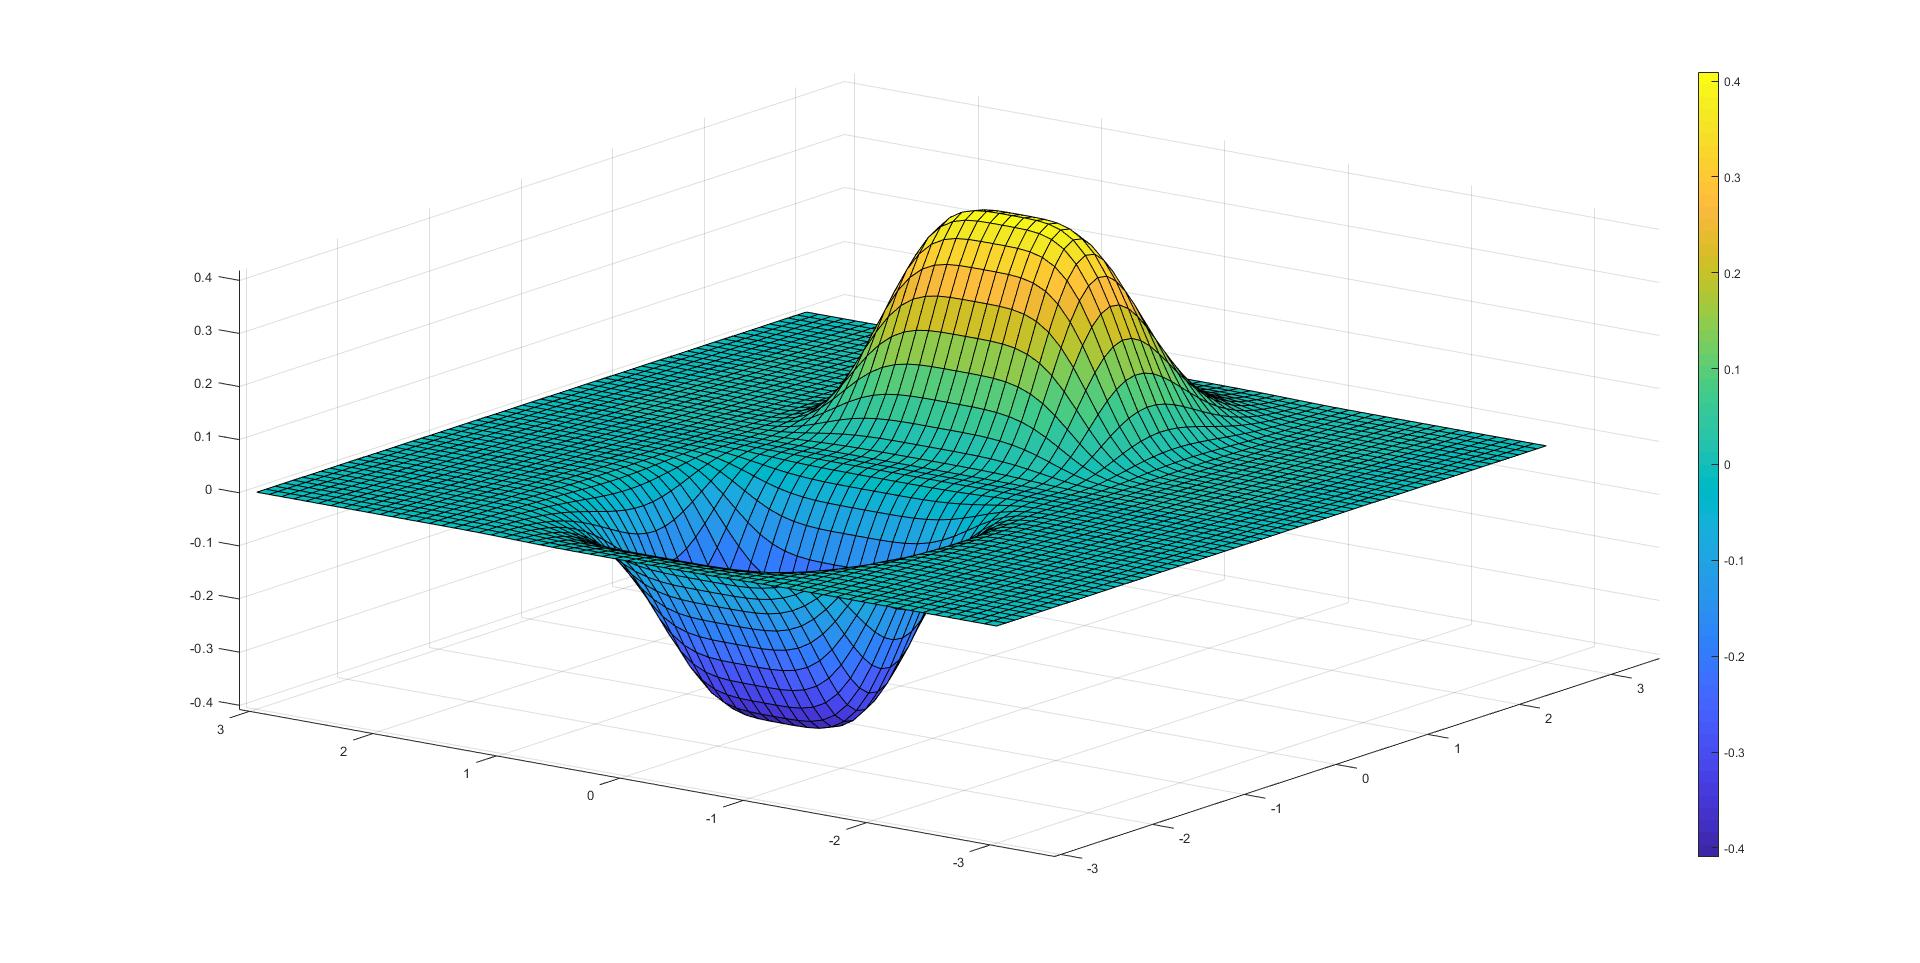
\includegraphics[width=130mm,scale=2]{functionF.jpg}
\end{figure*} 

Γραφική παράσταση της συνάρτησης 
\begin{equation*}
g(x,y) = x^4 + y^2 - 0.2sin(2πx) - 0.3cos(2πy)
\end{equation*}
\begin{figure*}[h!]	
     \centering  
     \advance\leftskip-0.2cm  
  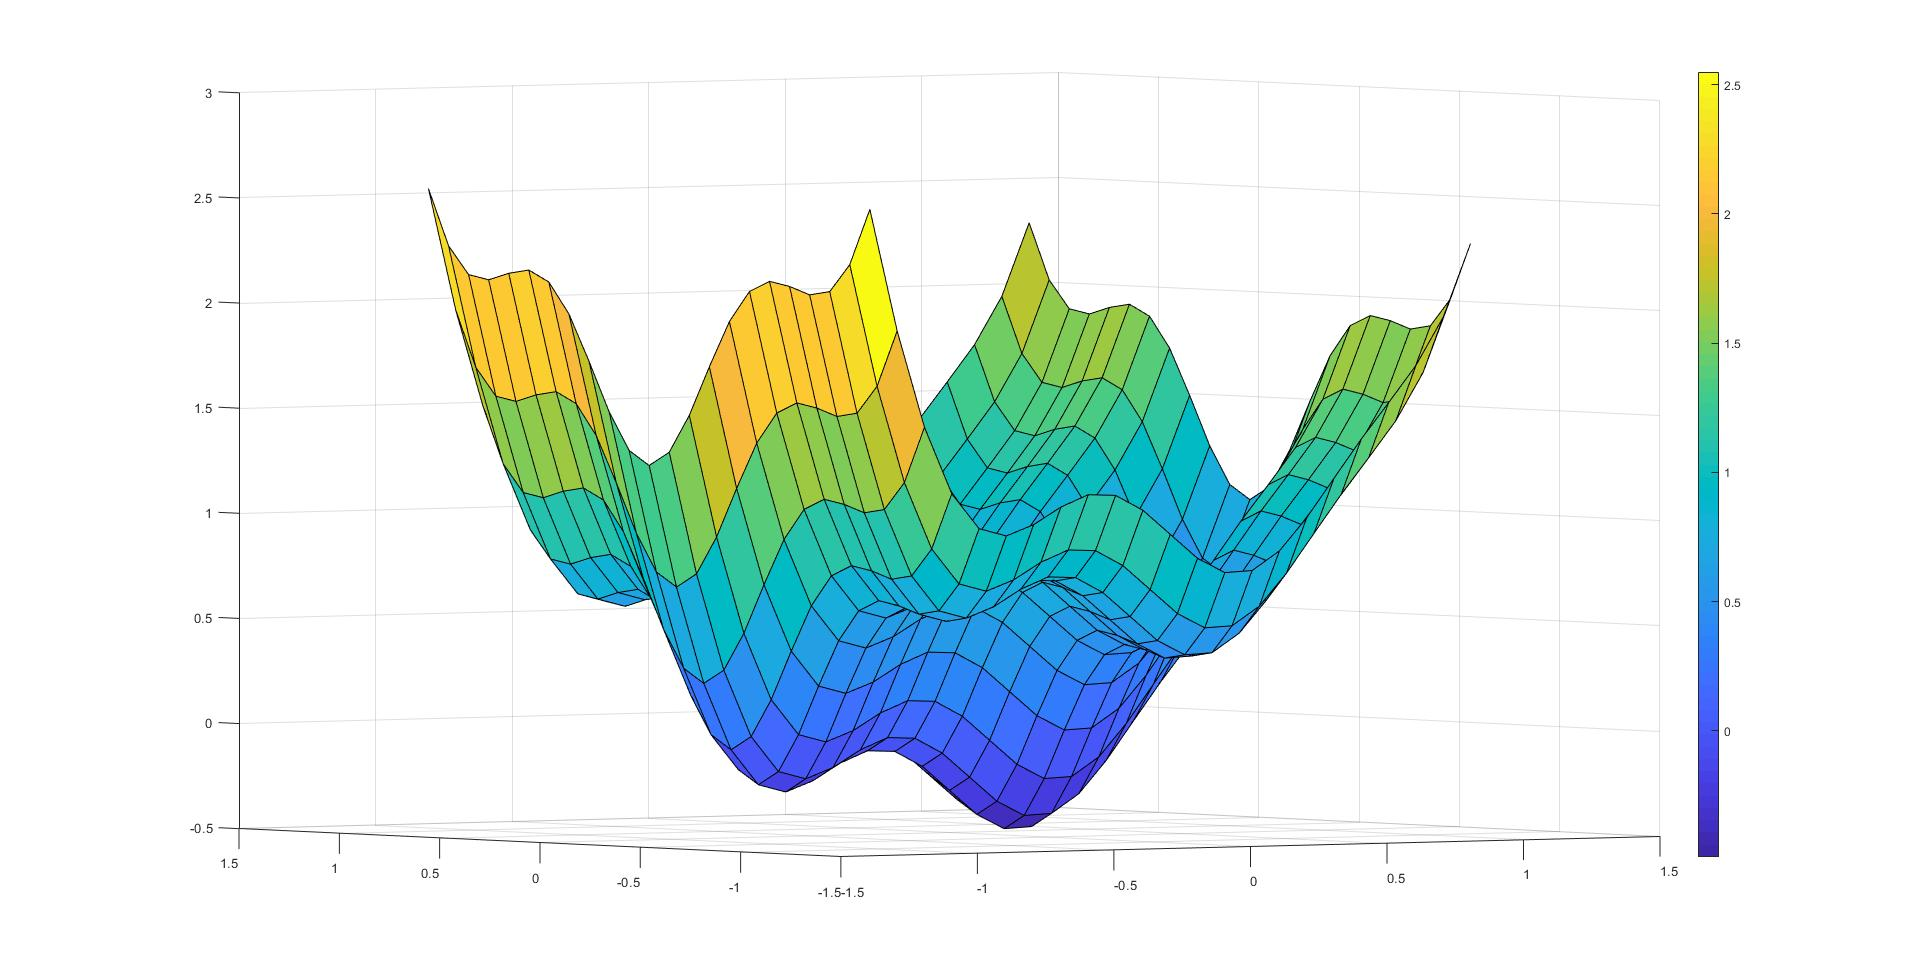
\includegraphics[width=130mm,scale=2]{functionG.jpg}
\end{figure*} 

\textit{o κώδικας των γραφικών παραστάσεων υπάρχει στο αρχείο \textbf{plot\_functions.m}}
\clearpage
\section*{Θέμα 2}
\subsection*{Ζητούμενα}
Στο πρώτο θέμα μας ζητείται να υλοποιήσουμε και να εφαρμόσουμε τη μέθοδο μέγιστης καθόδου (steepest descent) για να ελαχιστοποιήσουμε τις συναρτήσεις f και g παίρνοντας τα αρχικά σημεία i) (0,0), ii) (-1,-1), iii) (1,1).\\Το βήμα $γ_κ$ θα επιλεγεί:
\begin{itemize}
\item σταθερό της επιλογής μας
\item μεταβλητό τέτοιο ώστε σε κάθε επανάληψη να ελαχιστοποιείται η $f(x_k+g_k \cdot d_k )$ 
\item  βάσει του κανόνα Armijo
\end{itemize}
\subsection*{Περιγραφή αλγορίθμου}
Θεωρούμε το πρόβλημα ελαχιστοποίησης μιας συνάρτησης τουλάχιστον δυο φορές παραγωγίσιμης f, στην ιδέα της επαναληπτικής διαδικασίας η οποία έχει ως εξής:\\
Ξεκινάμε από το σημείο $x_0$ και παράγουμε διαδοχικά τα διανύσματα $x_1,x_2,..$ ώστε
\begin{equation*}
f(x_{k+1}) < f(x_k) \enspace k=0,1,2,...
\end{equation*} 
Ο αλγόριθμος υλοποιεί την ιδέα της επαναληπτικής καθόδου που μας οδηγεί σε ολοένα και βελτιωμένες τιμές της f, προς την ελαχιστοποίηση της.

\subsection*{Σταθερό γάμμα}
Θέτουμε ένα σταθερό $\boxed{γ=0.7}$ της επιλογής μας για την συνάρτηση f και εντός του αλγορίθμου κάνουμε τους απαραίτητους ελέγχους για να δούμε αν η επιλογή μας αυτή θα συγκλίνει σε κάποιο αποτέλεσμα. Όταν η τιμή του γ είναι πολύ μικρή τότε τα βήματα των επαναλήψεων για την εύρεση ελαχίστου αυξάνουν σημαντικά. Απο την άλλη η επιλογή ενος μεγάλου γ για το σύστημα προκαλεί αστάθεια καθώς με μεγάλο βήμα ο αλγόριθμος αδυνατεί να βρει τον ελάχιστο. Επίσης για την ακρίβεια e, δηλαδή πόσο κοντά θα είμαστε στο ελάχιστο επιλέξαμε αρκούντος μικρή τιμή $\boxed{e = 10^{-4}}$\\Πιο αναλυτικά, στο ελάχιστο η παράγωγος είναι μηδέν οπότε για να προσεγγίσουμε το ελάχιστο και να βρισκόμαστε κοντά του πρέπει η παράγωγος να είναι πολύ μικρή-σχεδόν μηδέν. 
Οπότε ξεκινώντας για γάμα 0.7 έχουμε τις εξής γραφικές για την μέθοδο μέγιστης καθόδου.
\clearpage
\subsubsection*{Αρχικό σημείο (0,0) για την συνάρτηση f}
\begin{figure*}[h!]	
     \centering  
     \advance\leftskip-0.2cm  
  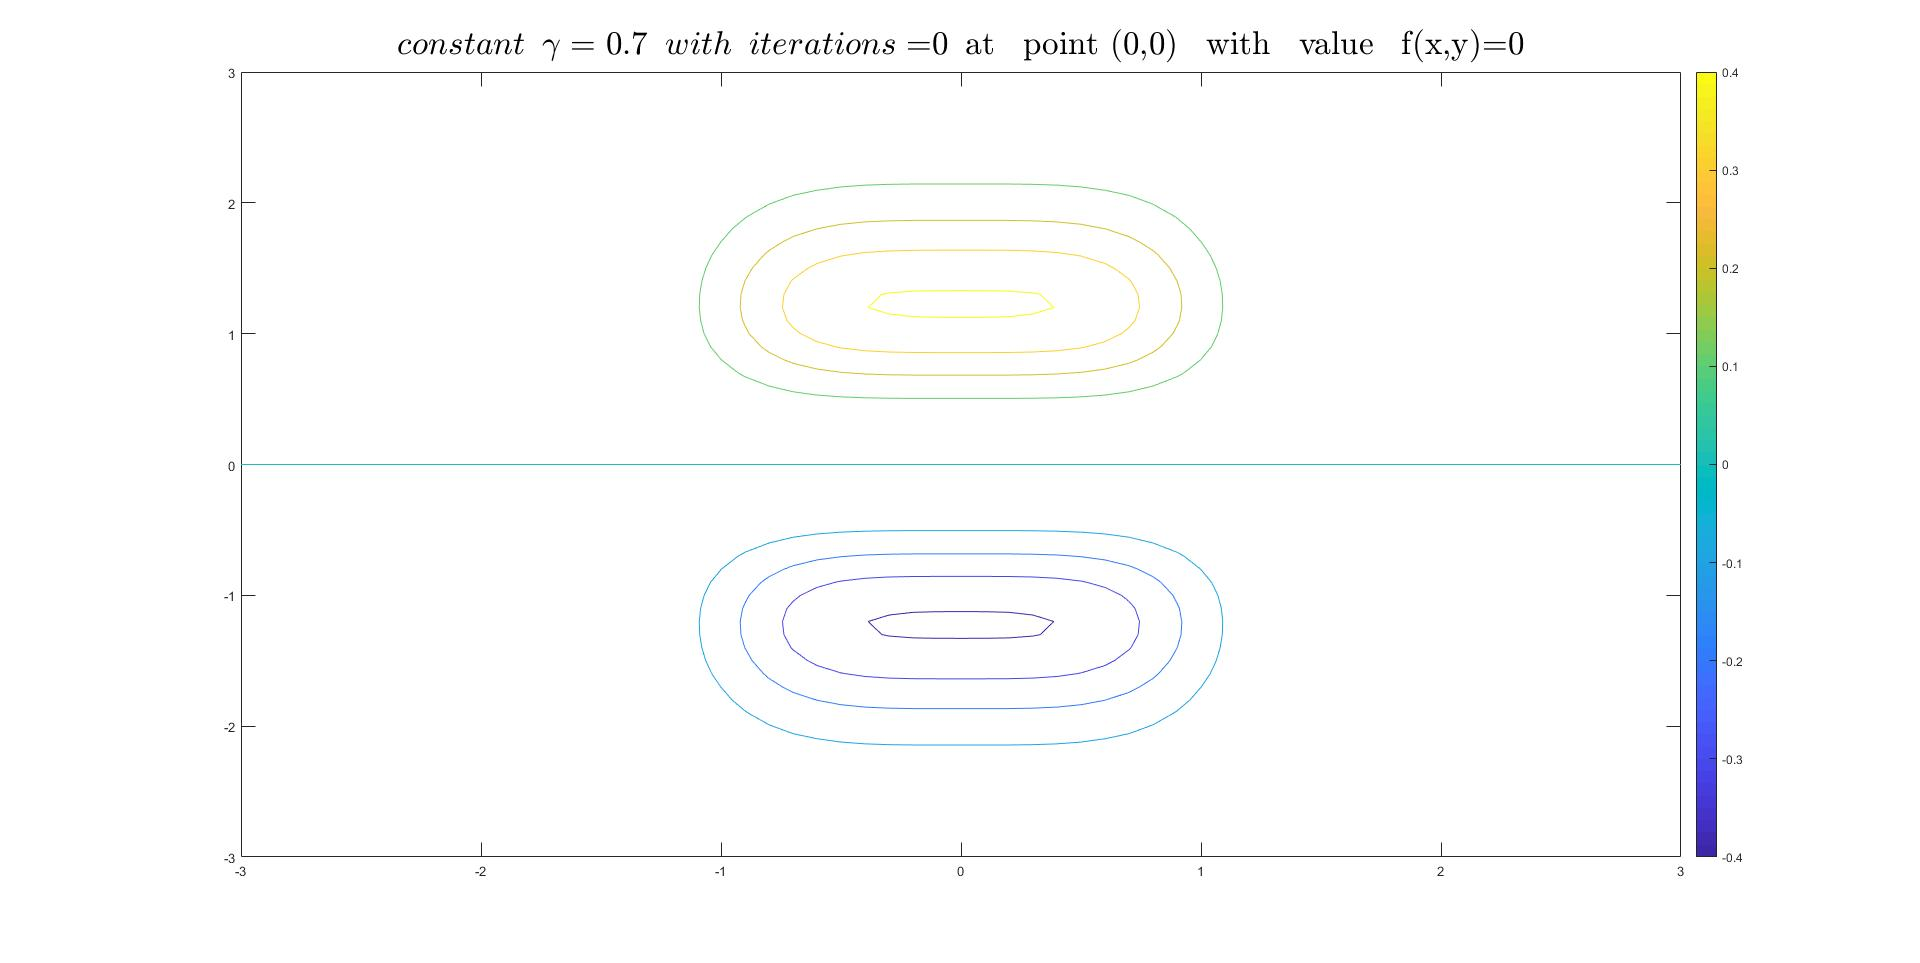
\includegraphics[width=140mm,scale=2]{t1a.jpg}
\end{figure*} 
Για αρχικό σημείο (0,0) η παράγωγος της f είναι μηδέν οπότε ο αλγόριθμος τερματίζεται πρόωρα και συνεπώς εγκλωβιζόμαστε στο σημείο f(x,y)=0.
\subsubsection*{Αρχικό σημείο (-1,-1) για την συνάρτηση f}
\begin{figure*}[h!]	
     \centering  
     \advance\leftskip-0.2cm  
  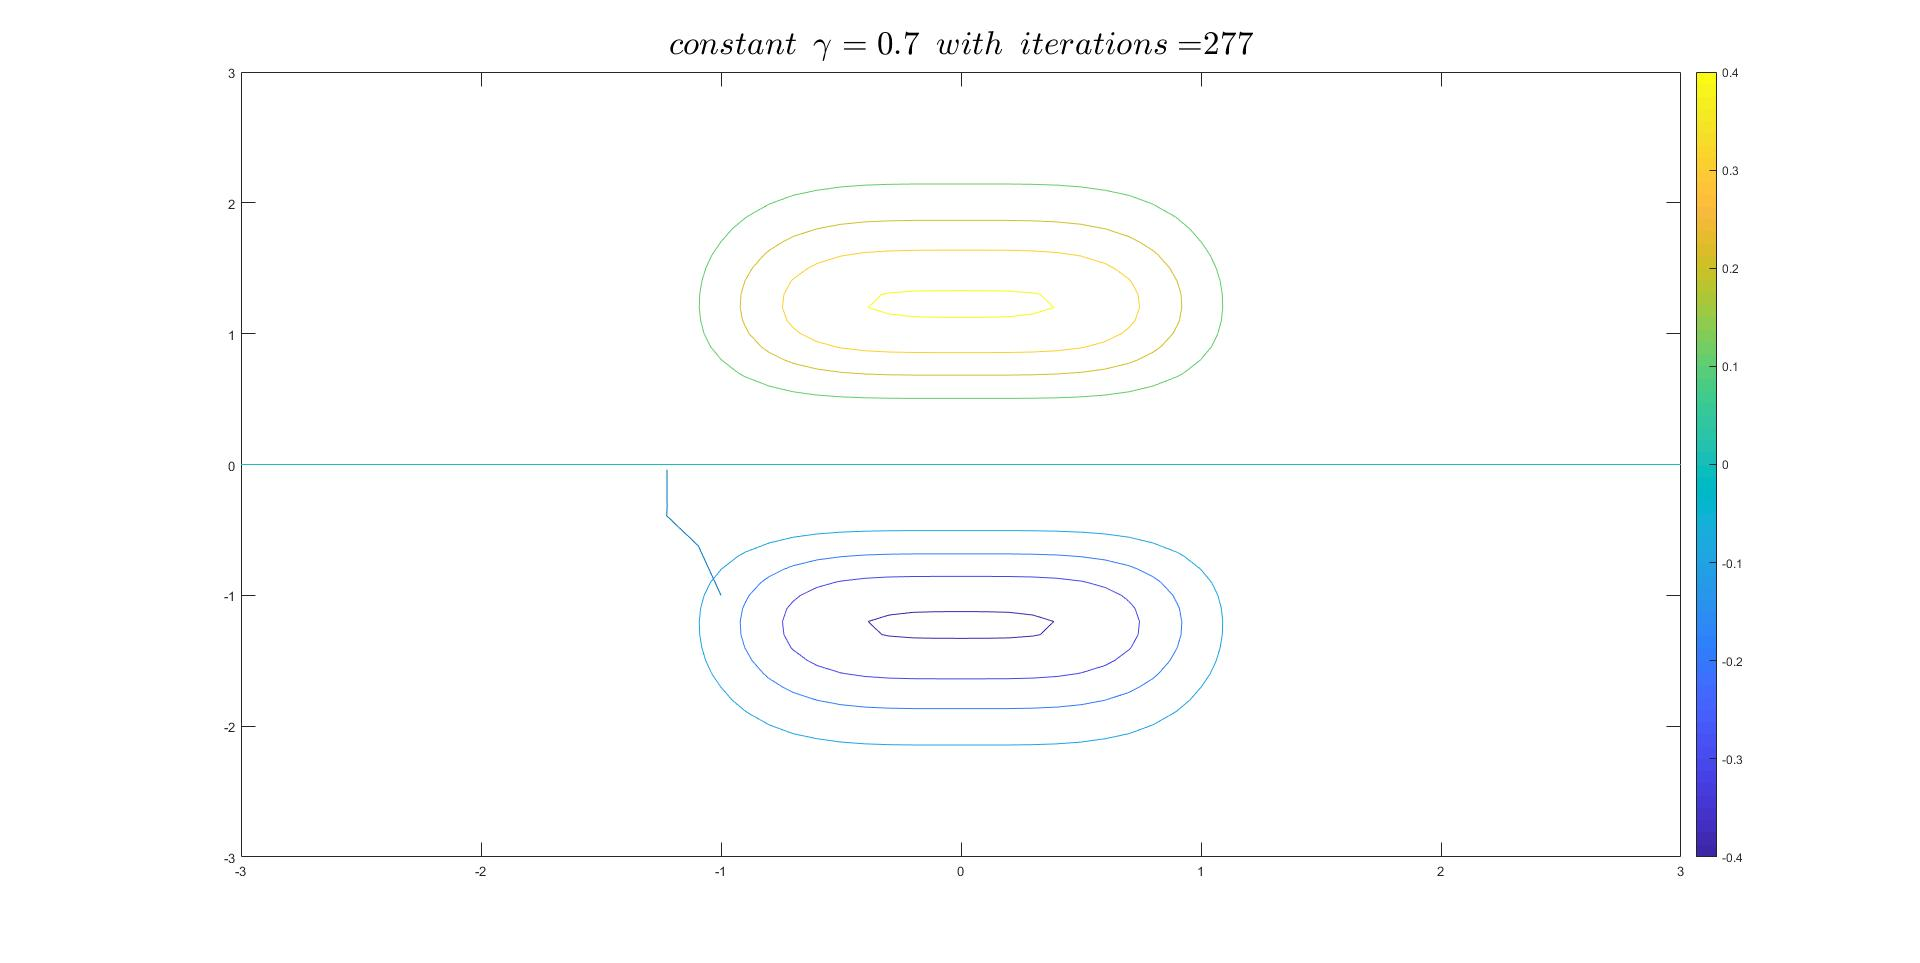
\includegraphics[width=140mm,scale=2]{t1b.jpg}
\end{figure*} 
Για αρχικό σημείο (-1,-1) μετά απο 277 επαναλήψεις καταλήγουμε σε τοπικό ελάχιστο (-1.22,-0.03) για  δοσμένη ακρίβεια e=$10^{-4}$ με τιμή f(x,y)=-0.409.
\clearpage
\subsubsection*{Αρχικό σημείο (1,1) για την συνάρτηση f}
\begin{figure*}[h!]	
     \centering  
     \advance\leftskip-0.2cm  
  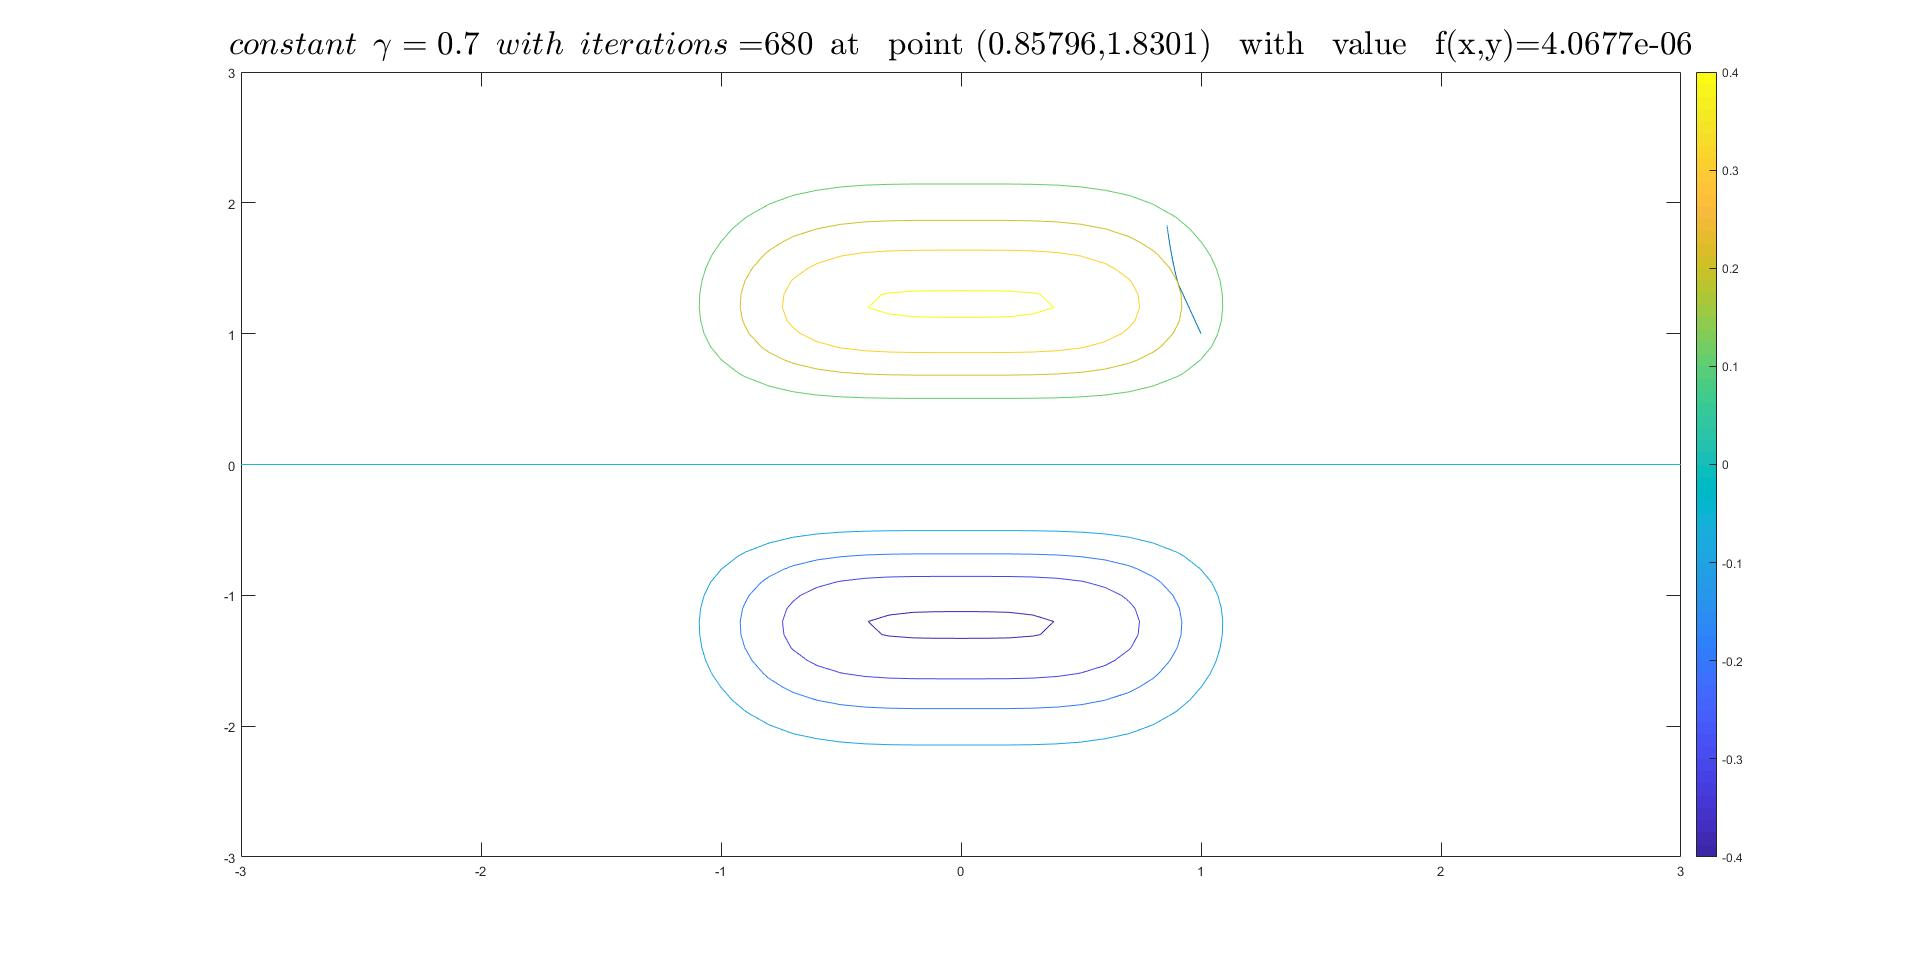
\includegraphics[width=140mm,scale=2]{t1c.jpg}
\end{figure*} 
Για αρχικό σημείο (1,1) μετά απο 680 επαναλήψεις καταλήγουμε σε τοπικό ελάχιστο (0.85,1.83) για δοσμένη ακρίβεια e=$10^{-4}$ με τιμή f(x,y)=4$\cdot 10^{-6}$.



\subsubsection*{Αρχικό σημείο (0,0) για την συνάρτηση g}
\begin{figure*}[h!]	
     \centering  
     \advance\leftskip-0.2cm  
  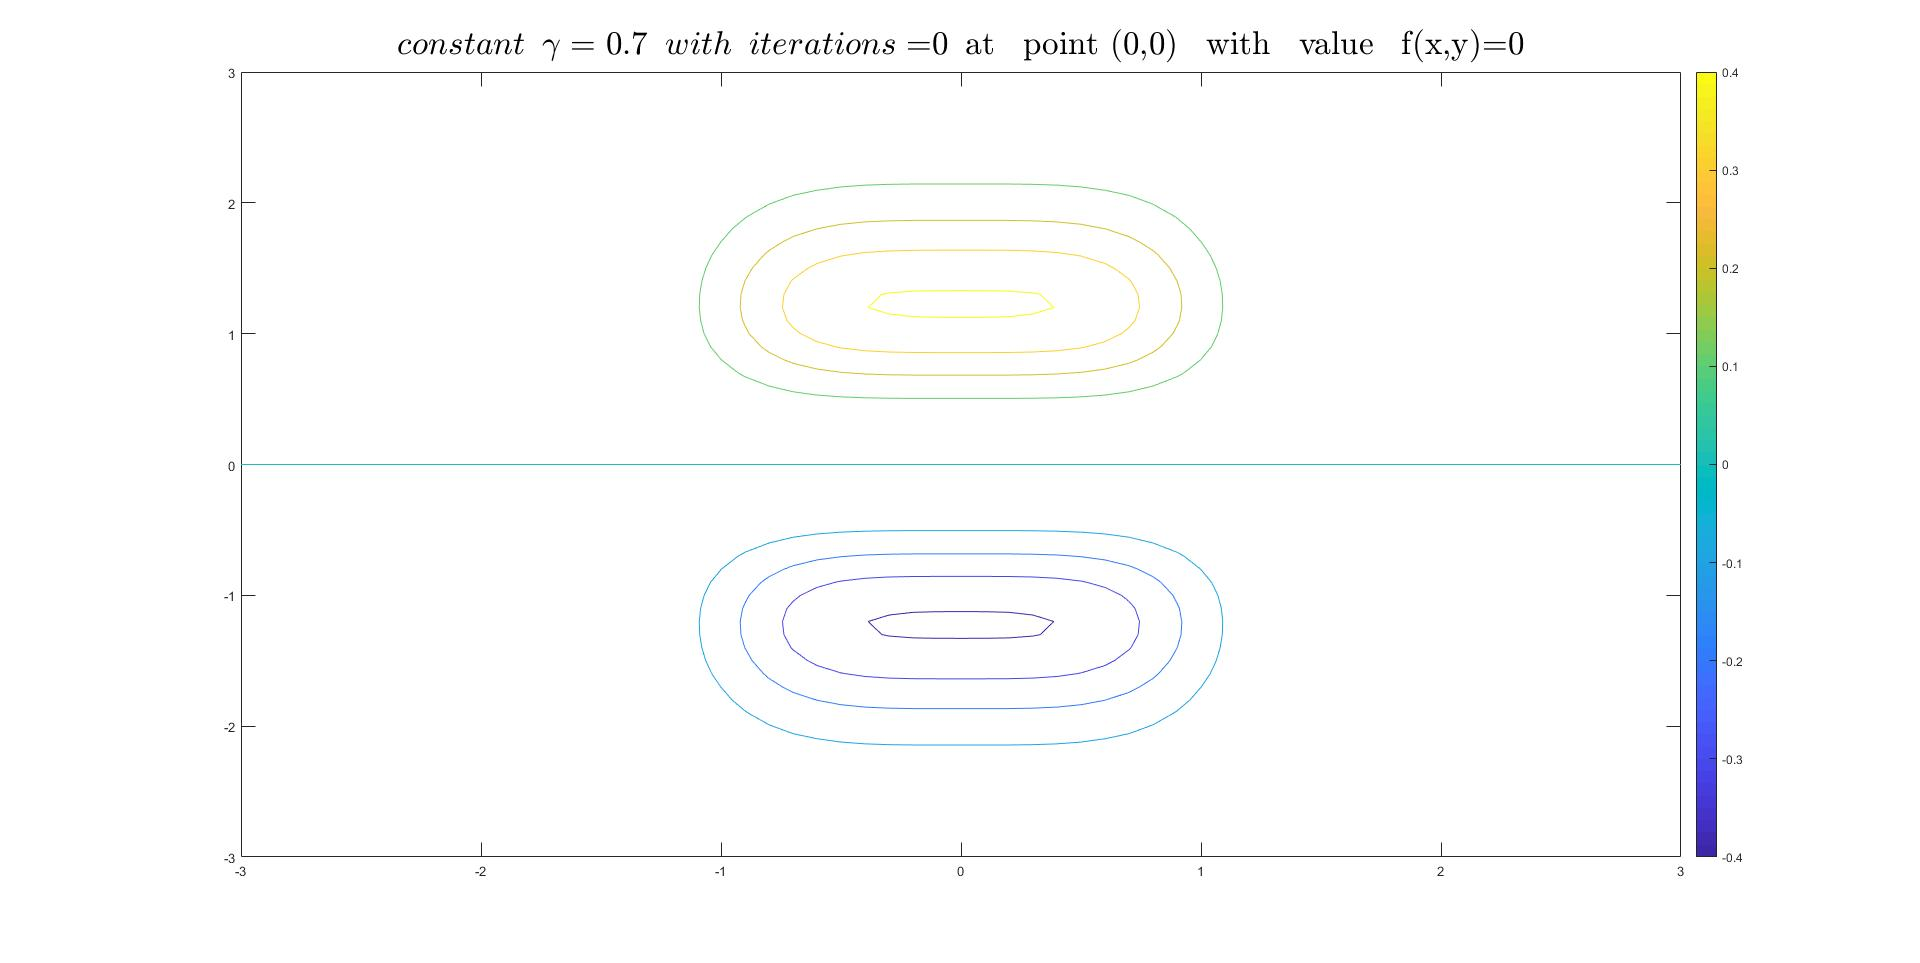
\includegraphics[width=140mm,scale=2]{t1a.jpg}
\end{figure*} 
Για αρχικό σημείο (0,0) μετά απο 680 επαναλήψεις καταλήγουμε σε τοπικό ελάχιστο (0.85,1.83) για δοσμένη ακρίβεια e=$10^{-4}$ με τιμή f(x,y)=4$\cdot 10^{-6}$.

\newpage 
\subsection*{Ελαχιστοποίηση $f(x_k+g_k \cdot d_k )$ }

 
\end{document}
